\lab{Applications}{Riemann Sphere and Mobius Transformations}{Riemann Sphere and Mobius Transformations}

\objective{Understand the Riemann Sphere in graphics applications.}

We have now examined several applications of complex numbers and functions.  In this lab we extend several of these ideas and develop some intuition about the Riemann sphere using visualization techniques in Python.

Recall that the complex numbers are an extension of the real numbers that include the imaginary numbers.  We extend them even further in this section and examine the extended complex numbers.  Similar to the extended real numbers, the extended complex numbers are our regular set of complex numbers with the addition of a point at infinity.  This allows us to examine, for example, certain quotients that are undefined on the standard complex numbers.

The Riemann sphere construction allows a compact and intuitive construction of the extended complex numbers.  Consider the standard complex plane, only now in 3-space instead of a 2 dimensional plane. Let the $x$-axis correspond to the real part of the complex numbers and let the $y$-axis correspond to the imaginary part.  Let $z=0$ for all $x$ and $y$. 

Now consider a the unit sphere centered at $(0,0,1)$ combined with the complex numbers in 3-space. We may map every point of the extended complex plane onto this sphere. Let infinity correspond to the point $(0,0,2)$ at the very top of the sphere. For all other points on the complex plane consider the line between the point on the complex plane and the point at the top of the sphere. Let each point of the complex plane map to the point where this line intersects with the surface of the sphere. Note that for any complex number, there is exactly one such point. This construction is illustrated below:

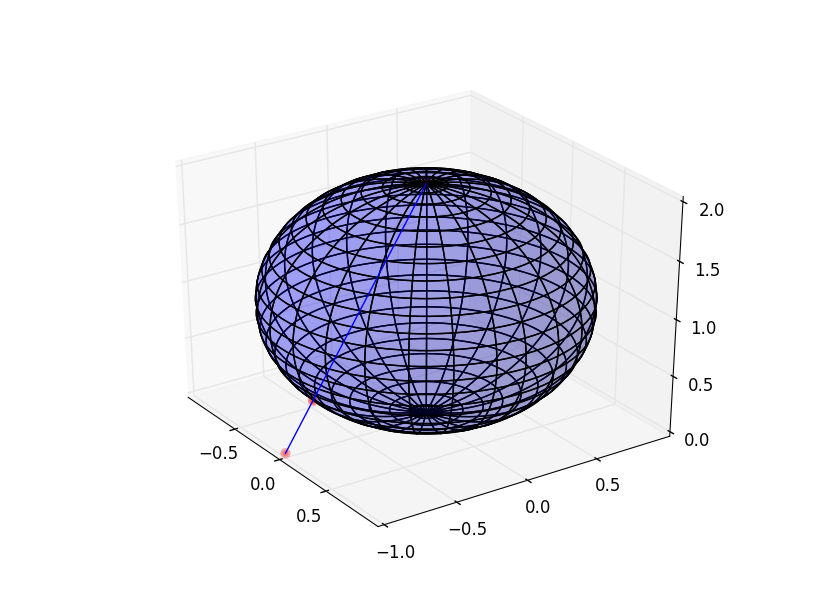
\includegraphics[width=120mm]{StereographicIllustration.png}

\begin{problem}  Write a function that, given a complex number, returns the coordinates of the corresponding point on the riemann sphere in 3-space.
\end{problem}

\begin{problem}
Write a function that, given the coordinates of a point on the Riemann Sphere, returns the corresponding point on the complex plane. If the input point is $(0,0,2)$ have your function return "infinity."
\end{problem}

\section*{Mobius Transformations}

Recall from the previous chapter that a conformal mapping is a complex function that preserves angles between lines.  We now examine a special kind of conformal mapping called a Mobius transformation.  We first give the definition of the Mobius transform, and then examine what sorts of transformations we can do with them.

\begin{definition}  A Mobius transformation is a any complex function of the form
\[
f(z) = \frac{az + b}{cz + d}
\]
 Where a, b, c, and d are complex numbers with the restriction that $ad \neq bc$.
\end{definition}

The Mobius transformation is versatile enough to include translations, rotations, magnifications, or any combination of the same, of shapes in the complex plane.  For example, if we wish to translate the unit disk on the complex plane and then magnify it two times, we would use the following transformation:
\[
PUT IT HERE
\]

{\bf PICTURE GOES HERE}

\begin{problem} Write a Python function that accepts arguments $a,b,c,$ and $d$.  Perform the corresponding Mobius transformation on a grid inside the box $[-1,1]\times[-i,i]$, and then visualize the box before and after the transformation on the same plot, but using different colors.
\end{problem}

What do these special transformations have to do with the Riemann sphere?  Recall from the conformal maps chapter that we can construct any point on the complex plane by drawing a line from infinity through a point on the Riemann sphere.  Consider the points on the sphere that can be used to construct the grid in the previous problem.

{\bf PICTURE GOES HERE}

It turns out that we can express any Mobius transformation as a translation or rotation of the Riemann sphere.  For example:

{\bf SEVERAL PICTURES WITH GOOD CAPTIONS GO HERE}

EXAMPLE OF HOW TO FIND THE TRANSFORMATION OF THE SPHERE HERE

\begin{problem}  Write a Python program that extends the previous problem to 3-dimensions.  Visualize the Mobius translation as a rotation/translation of the Riemann sphere.
\end{problem}



